
\section{Часть Савосина Артема}


\subsection{Первый прототип классификатора (Максим Макаров)}
Также, несмотря на то что это не входило в список моих задач, я решил попробовать создать первый прототип классификатора обработанных данных.
% Моими основными задачами были доработка мобильного приложения и создание классификатора обработанных данных.
Так как обработанные данные есть ни что иное, как фигура на плоскости, было рассмотрено несколько вариантов классификации этих самых данных:
\begin{enumerate}
    \item Классифицировать фигуры без какой-либо дополнительной обработки
    \item Нормировать фигуры по максимальному отклонению от точки (0; 0)
    \item Построить графики с помощью программной библиотеки mathplotlib, после чего классифицировать полученные изображения
\end{enumerate}
В связи с тем, что классификация изображений является весьма распространенной задачей, то было решено выбрать следующую стратегию: строить графики показаний акселерометра с помощью программной библиотеки mathplotlib и классифицировать полученные изображения.

Таким образом, возникли следующие подзадачи:
\begin{enumerate}
    \item Построить графики с помощью программной библиотеки mathplotlib
    \item Классифицировать полученные изображения, используя методы машинного обучения
    \item Добавить вывод предсказаний в мобильное приложение
\end{enumerate}
Благодаря лабораторным работам по линейной алгебре имелся достаточно богатый опыт использования программной библиотеки mathplotlib, поэтому построение графиков не составило труда. Однако, необходимо было избавиться от посторонних данных на графиках, таких как шкалы и вспомогательные сетки, а также привести все данные к единому формату: квадратные изображения строго определенного размера, одинаковый масштаб по оси абсцисс и по оси ординат.

\begin{figure}[H]
    \begin{center}
        \begin{tabular}{cc}
            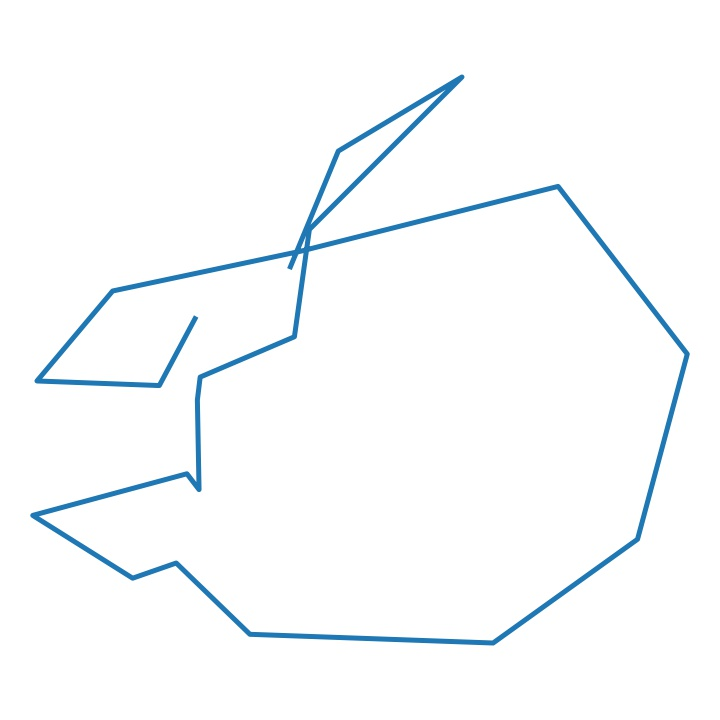
\includegraphics[width=0.4\textwidth]{max_kt2_images/image4.jpg} & 
            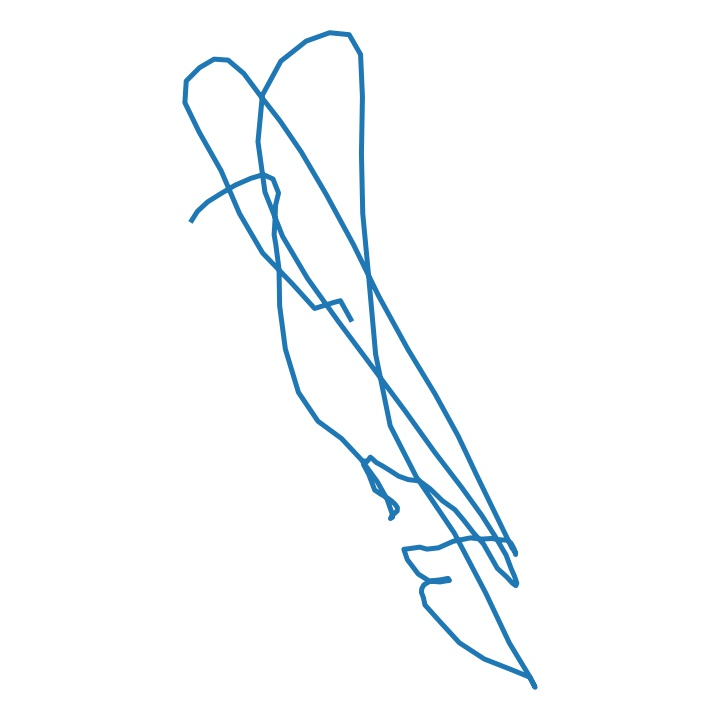
\includegraphics[width=0.4\textwidth]{max_kt2_images/image2.jpg} \\
        \end{tabular}
    \end{center}
    \caption{Примеры полученных изображений различных жестов: круг (слева), встряхивание (справа).}
\end{figure}

% Дополнительно, бонусом такого решения является то, что изображения нормируются по размеру автоматически.

Далее, я приступил к поиску подходящей программной библиотеки машинного обучения. Были рассмотрены следующие варианты:
\begin{enumerate}
    \item Theano -- библиотека численного вычисления в Python. Вычисления в Theano выражаются NumPy-подобным синтаксисом и компилируются для эффективных параллельных вычислений как на обычных CPU, так и на GPU.
    \item TensorFlow — открытая программная библиотека для машинного обучения, разработанная компанией Google для решения задач построения и тренировки нейронной сети с целью автоматического нахождения и классификации образов, достигая качества человеческого восприятия.
    \item Apache MXNet —  это программная платформа глубокого обучения с открытым исходным кодом, используемая для обучения и развертывания глубоких нейронных сетей.
\end{enumerate}

В связи с популярностью программной библиотеки TensorFlow и, как следствие, обилием готовых решений, основанных на ней, выбор был очевиден. Также данная библиотека является достаточно производительной, так как вся работа ведется с графами вычислений, операции с которыми, можно эффективно исполнять на некоторых типах процессоров.  Так как опыта работы с TensorFlow у меня не было совсем, первым делом было решено искать примеры проектов, сделанных на основе этой программной библиотеки. В процессе поиска я наткнулся на очень интересное решение от Google – Teachable Machine. Это инструмент, основанный на веб-технологиях, который делает обучение моделей быстрым, легким и доступным каждому, а также позволяет экспортировать полученные модели для интеграции в собственные решения.

\begin{figure}[H]
    \begin{center}
        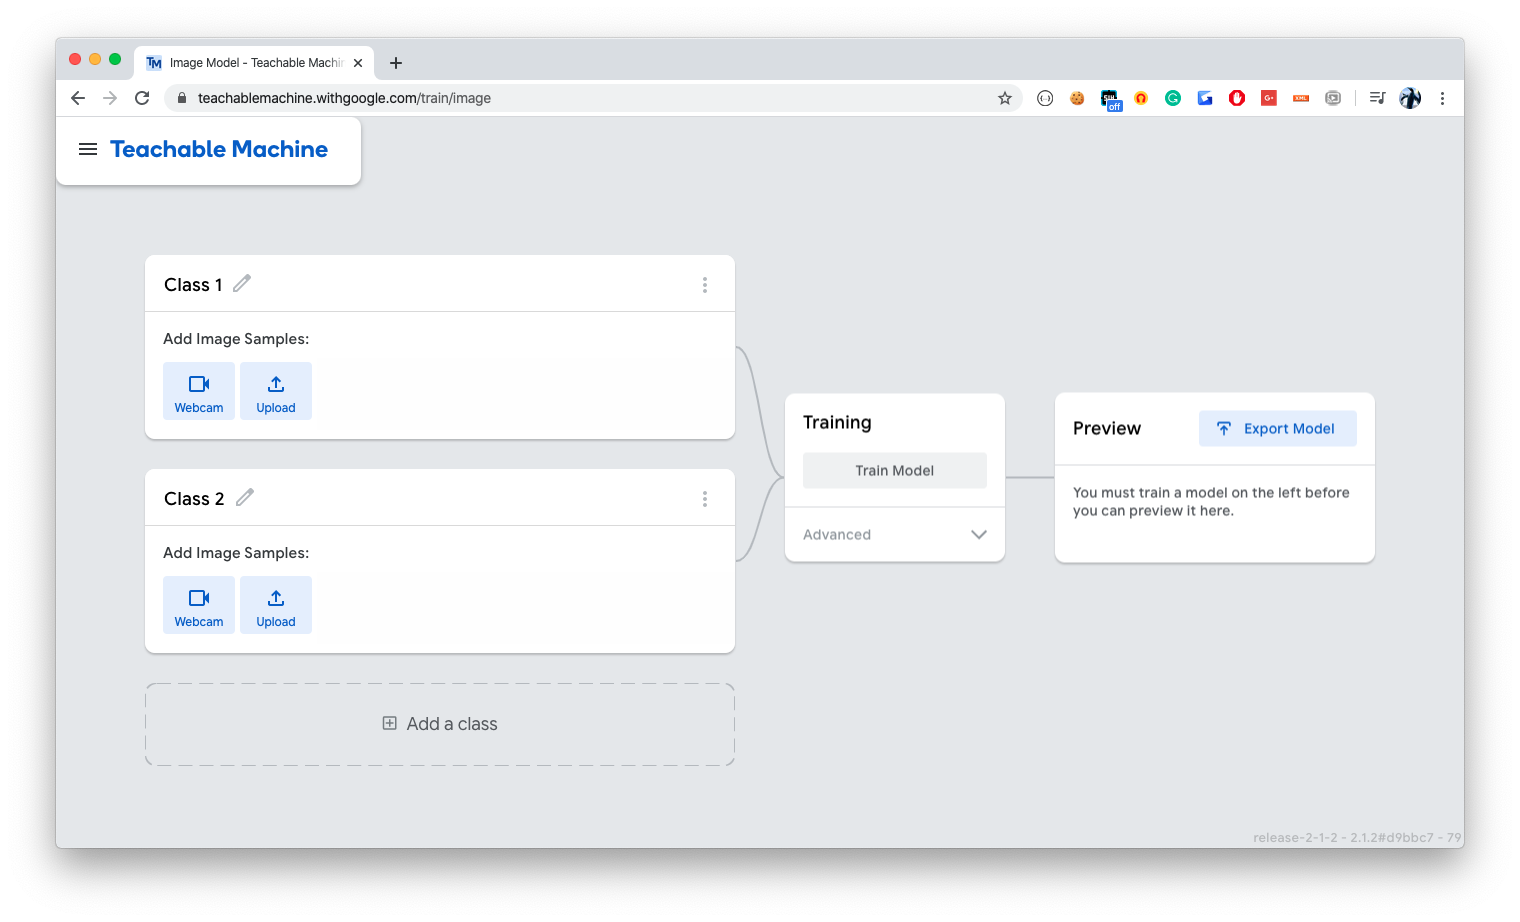
\includegraphics[width=0.8\textwidth]{max_kt2_images/image10.png}
    \end{center}
    \caption{Интерфейс программы “Teachable Machine”.}
\end{figure}

В программе предустановлены 3 модели: для распознавания изображений, аудиозаписей и поз. Нас интересует первая модель – это сверточная нейронная сеть. Данный тип искусственных нейронных нейронных сетей хорошо зарекомендовал себя в задачах распознавания образов. Главное отличие сверточных нейронных сетей от обыкноневенного перцептрона, то есть полносвязной нейронной сети, в том, что она обучается на основе карт признаков, которые формируются в результате операций свертки матрицами весов различных фильтров. Сами же матрицы весов корректируются в процессе обучения методом обратного распространения ошибки.

\begin{figure}[H]
    \begin{center}
        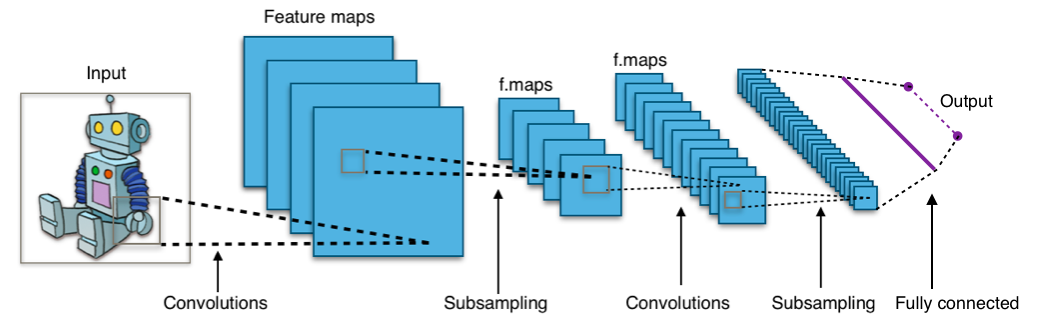
\includegraphics[width=0.8\textwidth]{max_kt2_images/image7.png}
    \end{center}
    \caption{Типовая архитектура сверточной нейронной сети.}
\end{figure}

% Принцип работы Teachable Machine прост: в левом меню создаются классы и для каждого загружается набор тренировочных изображений или аудиозаписей в зависимости от выбранного ранее типа модели. При необходимости можно указать дополнительные параметры обучения (скорость обучения, количество эпох и т.д.), однако, как выяснилось позже, стандартные параметры обучения позволяют добиться достаточно неплохих результатов. Затем, полученную модель можно экспортировать в формате “.h5”.

Далее, нужно было определиться с классами движений. После совещания с другими участниками команды, мы остановились на том, что система будет уметь распознавать три типа жестов: круг, квадрат и встряхивание. Недолго думая, один из участников команды приступил к сбору датасета и уже через пару часов, в моих руках было 15 экземпляров “кругов”, 14 “квадратов” и столько же “встряхиваний”. Далее, данный набор данных был загружен в Teachable Machine, а также была запущена тренировка со стандартными настройками (50 эпох, batch size = 16, скорость обучения = 0,001).  После чего, модель была экспортирована для использования вместе с интерпретируемым языком программирования Python 3. Сразу же захотелось протестировать данную модель: из другого набора данных были выбраны несколько записанных ранее жестов в виде графиков, которые после стали входными данными для алгоритма распознавания. Были получены следующие результаты:

\begin{figure}[H]
    \begin{center}
        \begin{tabular}{cc}
            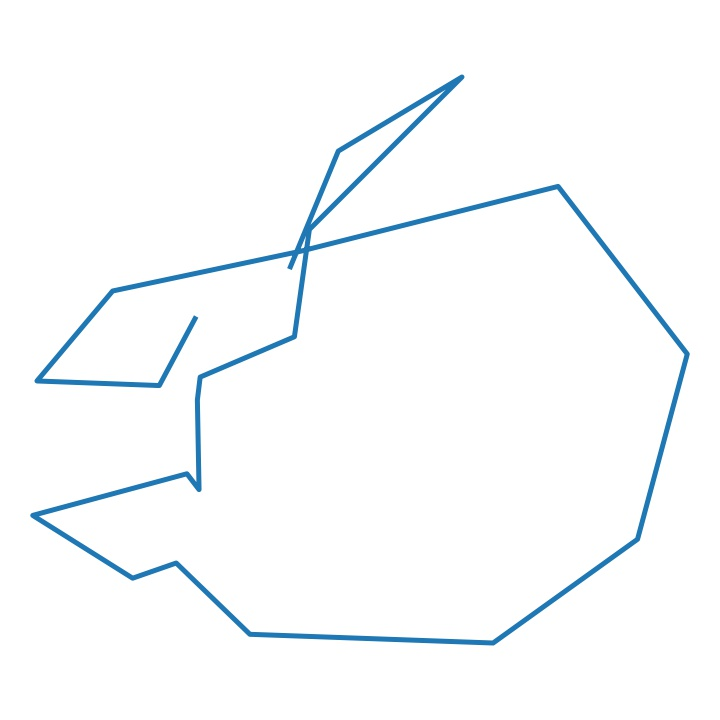
\includegraphics[width=0.35\textwidth]{max_kt2_images/image4.jpg} & 
            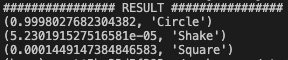
\includegraphics[width=0.35\textwidth]{max_kt2_images/image11.png} \\
        \end{tabular}
    \end{center}
    \caption{Исходное изображение круга (слева) и результат работы алгоритма (справа).}
\end{figure}

\begin{figure}[H]
    \begin{center}
        \begin{tabular}{cc}
            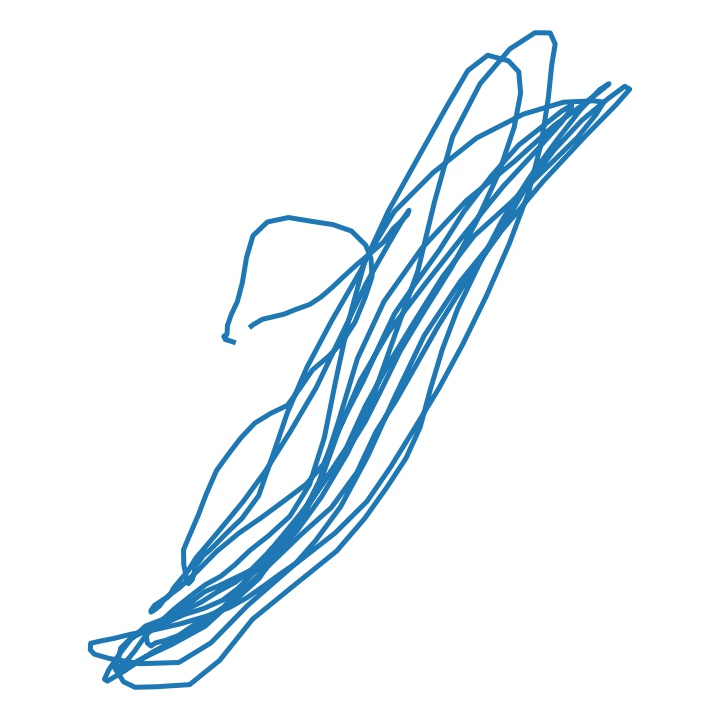
\includegraphics[width=0.35\textwidth]{max_kt2_images/image9.jpg} & 
            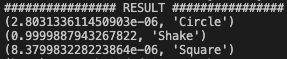
\includegraphics[width=0.35\textwidth]{max_kt2_images/image8.png} \\
        \end{tabular}
    \end{center}
    \caption{Исходное изображение встряхивания (слева) и результат работы алгоритма (справа).}
\end{figure}

\begin{figure}[H]
    \begin{center}
        \begin{tabular}{cc}
            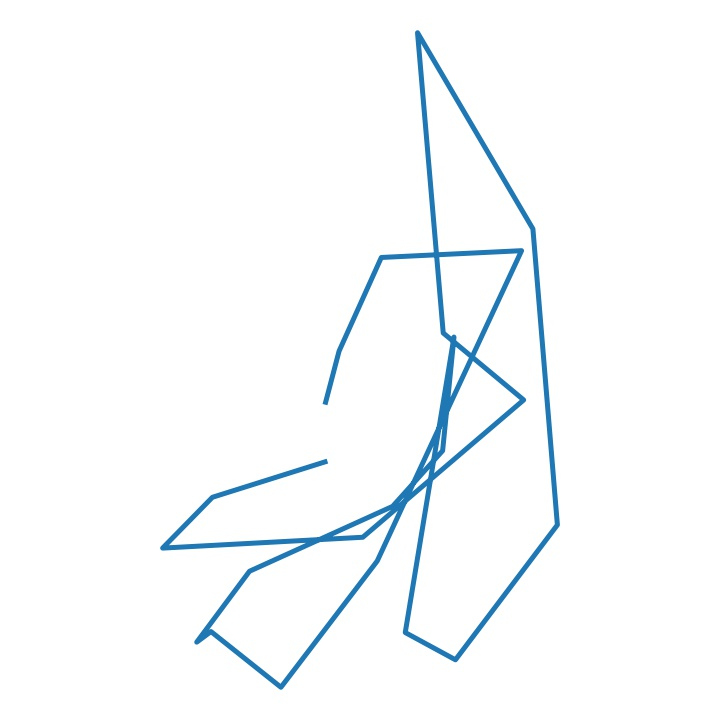
\includegraphics[width=0.35\textwidth]{max_kt2_images/image3.jpg} & 
            
\includegraphics[width=0.35\textwidth]{max_kt2_images/image1.png} \\
        \end{tabular}
    \end{center}
    \caption{Исходное изображение квадрата (слева) и результат работы алгоритма (справа).}
\end{figure}


\subsection{Теоретическая часть. Описание выбранных и/или разработанных методов, алгоритмов, моделей данных, методик и т.п.}

\subsubsection{Сбор данных.}
Для работы по обучению модели, классифицирующей жесты, необходимо было собрать данные с этими жестами. Предположив, что жесты пользователей будут различаться в зависимости от их возраста, пола, физических особенностей, было принято решение собрать записи движений разных пользователей. Удалось записать движения 10 пользователей, 6 персон женского пола, 4 мужского, 5 пользователей старшей возрастной группы.
Суммарно мы получили 600 различных движений.
Данные заранее были случайным образом разбиты на две группы - для тренировки модели и для проверки ее точности.

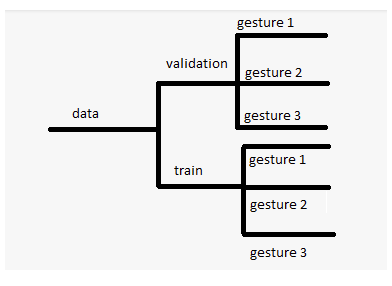
\includegraphics[scale = 1]{images_sav/data.png}

\subsubsection{Наилучшая плоскость для проекции.}

На вход ко мне подаются пред обработанные данные - отфильтрованные, усредненные по тактам (если их было несколько). Данные задаются массивом из 3-х мерных векторов, которые выглядят вот так
\begin{figure}[H]
\center{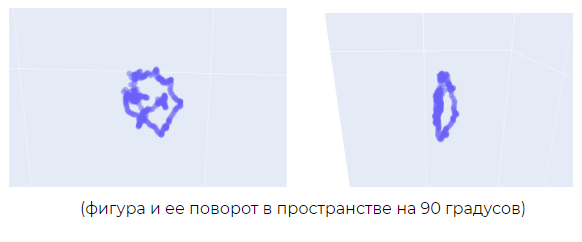
\includegraphics[scale = 0.5]{images_sav/3d_fig.png}}
\end{figure}
Для наших данных хотим найти такую двумерную плоскость, что на ней отобразится максимум информации про наше движение - минимум точек совпадут с друг с другом и 2d картинка останется максимально похожей на свой 3d аналог. 

Уравнение плоскости задается уравнением $ax+by+c=z$. 
Задаем систему уравнений 
\begin{figure}[H]
\center{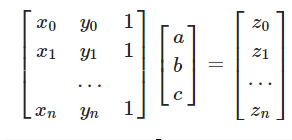
\includegraphics[scale = 1]{images_sav/math1.png}}
\end{figure}
где $(x_i, y_i, z_i)$  - это векторы из массива, а (a, b, c) - нормаль, которую нам нужно найти. В силу того, что в массиве у нас явно больше, чем 3 вектора, система будет переполненной, и нам нужно будет использовать псевдообратную матрицу 
\begin{figure}[H]
\center{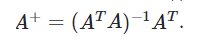
\includegraphics[scale = 1]{images_sav/math2.png}}
\end{figure}
Таким образом нормаль плоскости находится по формуле
\begin{figure}[H]
\center{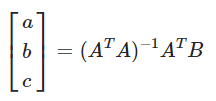
\includegraphics[scale = 1]{images_sav/math3.png}}
\end{figure}
\begin{figure}[H]
\center{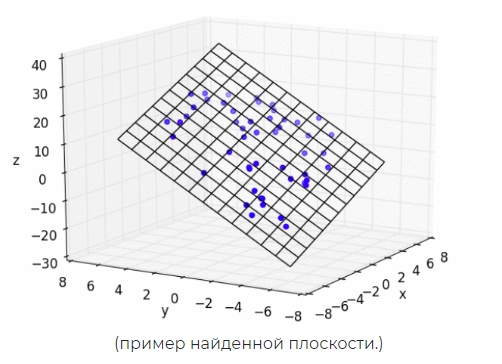
\includegraphics[scale = 1]{images_sav/flat_plot.png}}
\end{figure}
Таким образом мы нашли нормаль для подходящей плоскости. Теперь остается только стандартным способом найти проекцию всех точек на эту плоскость и получить плоскую картинку движения.
\begin{figure}[H]
\center{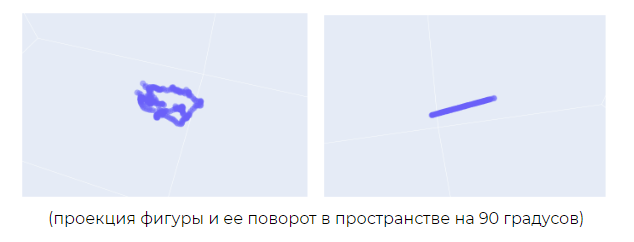
\includegraphics[scale = 1]{images_sav/2d_fig.png}}
\end{figure}
Получилась плоская фигура, находящаяся в 3D пространстве, из нее получаем 2D изображение.
\begin{figure}[H]
\center{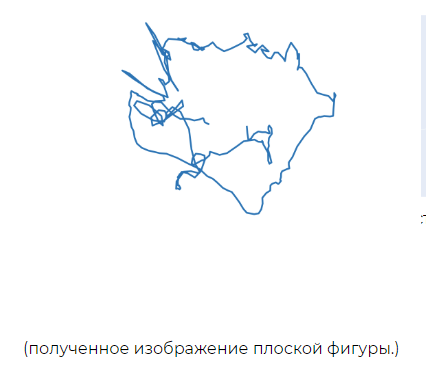
\includegraphics[scale = 1]{images_sav/2d_fig_img.png}}
\end{figure}
\subsubsection{Классификация данных.}

После проделанной выше работы - получение, фильтрация, выделение такта, нахождение среднего движения из нескольких тактов, перенос 3-х мерных данных в 2-х мерное изображение, остается только классифицировать полученный набор данных. 
\begin{figure}[H]
\center{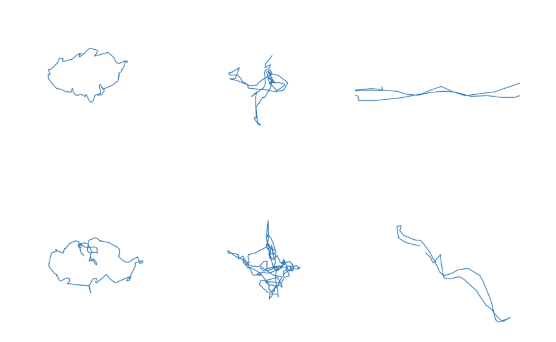
\includegraphics[scale = 1]{images_sav/data_examples.png}}
\end{figure}
Выше представлены примеры данных, полученных в ходе работы. Каждый ряд картинок отображает один из классов движений - круг, квадрат, встряска. Человеческий мозг легко бы справился с задачей распознать и классифицировать новое изображение, основываясь даже на таком небольшом количестве примеров. Легко можно заметить, что в классе кругов изображения будут примерно похожи на овалы, в классе квадратов можно наблюдать фигуру схожую с крестом, а изображения из класса встрясок похожи на линию. К сожалению, то, что понятно человеку, не так просто объяснить машине. Нашей команде понадобилось бы большое количество времени, чтобы описать все условия принадлежности той или иной фигуры к определенному классу, если бы нам вообще удалось это сделать. Решить задачу классификации мы сможем, применив сверточную нейронную сеть.
\subsubsection{Что такое нейронная сеть?}
Это математическая модель, изобретенная в ходе изучения работы мозга и попытке смоделировать его поведение. 
Мозг человека состоит из нейронов, соединенных между собой каналами, по которым передается электрический импульс. Нейроны получают сигналы от многих других нейронов, обрабатывают их, и посылают новый сигнал. 
Когда мы видим какое-то изображение, в зрительной коре головного мозга активируются строго определенные участки, которые передают сигнал далее, где он обрабатывается, и мы понимаем, что перед нами, скажем, круг, а не квадрат.
Компьютерная нейронная сеть - это попытка хотя бы частично воссоздать процесс, происходящий в голове в момент распознавания картинки.  Простая нейронная сеть состоит из нескольких слоёв. 
\begin{figure}[H]
\center{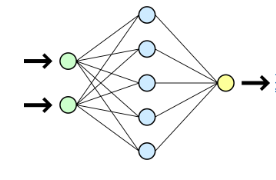
\includegraphics[scale = 1]{images_sav/neuro.png}}
\end{figure}

Входной слой (зеленый) - это “глаза” нашей сети.
 Скрытый слой (синий)
Выходной слой (желтый) - в этом слое ровно столько нейронов, сколько мы имеем классов изображений. А сила сигнала на том или ином нейроне говорит о том, насколько сильно входной объект похож на объект, за который отвечает этот нейрон.
\subsubsection{Что такое сверточная нейронная сеть?}
СНС состоит из разных видов слоев: сверточные (convolutional) слои, субдискретизирующие (subsampling, подвыборка) слои и слои «обычной» нейронной сети – персептрона.
Главное отличие такой сети - наличие сверточных слоев. Перед тем, как тренировать модель, изображение будет пропущено через ряд сверток - некоторое количество фильтров, позволяющих выделить характерные признаки изображения.
\subsubsection{Так как же сеть классифицирует изображения?}
Как я уже отмечал ранее, нейроны связаны между собой каналами. 
Входные нейроны связываются со скрытыми, скрытые с выходными. На каждой такой связи расставляются веса - насколько сильно важен для следующего нейрона входящий в него по этой связи нейрон. Далее каждый нейрон производит некоторые вычисления внутри себя, и передает сигнал далее.
Когда на вход подается изображение, входные нейроны задействуются, а сила сигнала, передаваемого ими, зависит от того, насколько яркая картинка в этом месте. Сигнал передается далее, происходят вычисления во внутренних слоях. После этого на каких-то выходных нейронах появится сигнал. Мы понимаем, какие выходные нейроны активны, и насколько они активны, и делаем вывод о принадлежности изображения к тому или иному классу.
\subsubsection{Тренировка нейронной сети.}
Нужно отметить, что при создании сети, веса между нейронами расставляются случайно - они никак не связаны с изображениями, которые мы хотим классифицировать. Далее мы прогоняем через такую сеть наши данные, и выявляем ошибки. На основе этих ошибок меняются веса связей, и мы снова прогоняем наши данные и смотрим, насколько хорошо классифицируется. Потом еще раз вносим коррективы в веса связей, и так далее. На каждом шаге обучения веса меняются с помощью функции оптимизации.


\subsubsection{Модель}

В нашем проекте используется библиотека tensorflow, позволяющая быстро создать и обучить собственную сверточную нейронную сеть. 

Для начала про данные - входные изображения разделены в пропорции 2 к 1 на тренировочные и валидационные. На первых модель обучается, вторые нужны для проверки на переобученность модели. 
Используя библиотеку keras preprocessing, мы нормируем все изображения так, чтобы входная матрица принимала цветовые значения не от 0 до 255, а от 0 до 1. Это требуется по причине того, что сети удобнее работать со значениями от 0 до 1. Далее в тренировочные данные добавляются измененные версии тренировочных файлов - изображения, повернутые на 45 градусов, Этот шаг нужен для того, чтобы избежать переобучения модели - ведь движения, записанные новым пользователем могут отличаться от собранных. 
Далее поговорим о самой модели и слоях, из которых она состоит
\begin{figure}[H]
\center{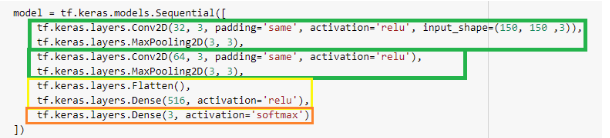
\includegraphics[scale = 1]{images_sav/model.png}}
\end{figure}
Входной слой состоит сверточного слоя ,который будет генерировать 32 фильтра для выделения параметров, за которым следует слой MaxPooling, который выделяет один, самый сильный сигнал из группы 3 на 3 и оставляет его, что позволяет значительно уменьшить изображение, сохранив его главные детали.  Далее повторим процесс, добавив новый сверточный слоев с большим количеством фильтров, таким образом, разбирая наше изображение на большое количество маленьких параметров, из которых складывается представление о фигуре.
Далее следуют слои обычной нейронной сети, с еще 516 фильтрами.
Последний слой состоит из 3 нейронов (по количеству классов) и активатора softmax. Активатор выбирает максимальное значение из трех нейронов, и присваивает ему весь сигнал, остальные нейроны будут пустыми. 

Про точность модели 
на финальном шаге обучения точность модели на обучаемых данных составила 97,92 процентов , а на независимых данных модель смогла угадать все 100 процентов представленных изображений. 
За два шага до этого модель укладывала 100 процентов всех тренировочных данных. \newline
Epoch 18/20 \newline
accuracy: 1.0000 - val-accuracy: 1.0000 \newline
Epoch 19/20\newline
accuracy: 1.0000 - val-accuracy: 0.9792\newline
Epoch 20/20\newline
accuracy: 1.0000 - val-accuracy: 0.9792\newline
\begin{figure}[H]
\center{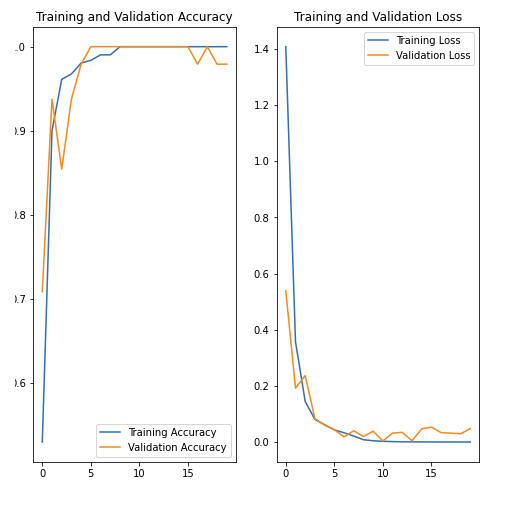
\includegraphics[scale = 1]{images_sav/accuracy.png}}
\end{figure}
\subsection{Описание вычислительного эксперимента -- план эксперимента, инструменты и средства его проведения, полученные результаты, их анализ и оценка}
Для определения и выявления наиболее подходящей модели для наших данных, мне пришлось провести ряд экспериментов - я выбирал разные функции оптимизации, менял количество и свойства слоев. 
Первой пробой была простая модель, состоящая из двух сверточных слоев.

\begin{figure}[H]
\center{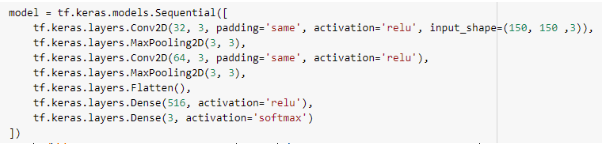
\includegraphics[scale = 1]{images_sav/model1.png}}
\end{figure}

На ней я использовал 4 функции оптимизации

\begin{itemize}
	\item Оптимизация Адама - это метод стохастического градиентного спуска, основанный на адаптивной оценке моментов первого и второго порядка.
	\item Adagrad - это оптимизатор с частотой обучения, зависящей от параметров, которая адаптируется в зависимости от того, как часто параметр обновляется во время обучения. Чем больше обновлений получает параметр, тем меньше обновлений.
	\item SGD - Стохастический градиентный спуск и оптимизатор импульса.
	\item Rmsprop
\end{itemize}

Данные генерировались с помощью простой функции, которая переводила матрицу со значениями от 0 до 255 в значения от 0 до 1.

\begin{figure}[H]
\center{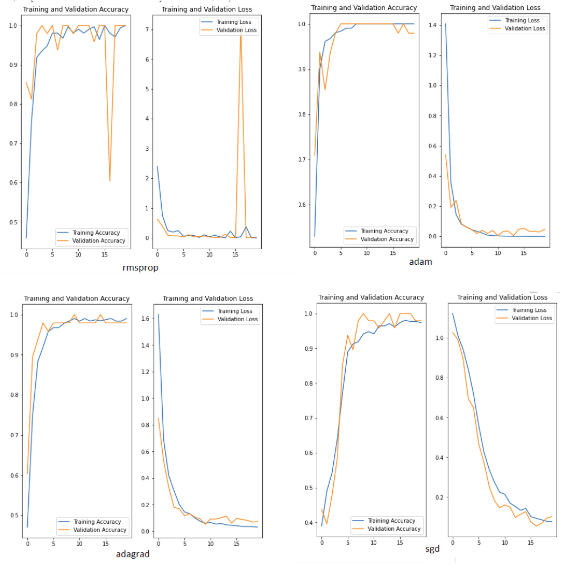
\includegraphics[scale = 0.6]{images_sav/exp1.png}}
\end{figure}
Заметим, что все модели показывают довольно неплохую точность - распознавание тренировочных данных не ниже 99 процентов, валидационных - 95. Главное отличие в скорости достижения высокой точности и потерях нейронов в ходе обучения. Лучше всего себя показала модель с функцией оптимизации adam.

Обычно, при обучении нейронной сети главной проблемой является переобучение, в результате которого модель начинает очень хорошо распознавать изображения, на которых она обучалась, и гораздо хуже распознает новые изображения. Проверим, что будет с нашими моделями, если мы добавим в них методы, противодействующие переобучению. 

Добавим еще один сверточный слой и введем новые слои Dropout, которые выкидывают 20 процентов обученных нейронов на каждом шаге, что уменьшает риск переобучения.  
\begin{figure}[H]
\center{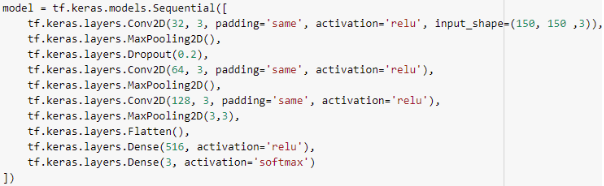
\includegraphics[scale = 1]{images_sav/model2.png}}
\end{figure}
Далее проверяем точность этих моделей на тех же 4 функциях.

\begin{figure}[H]
\center{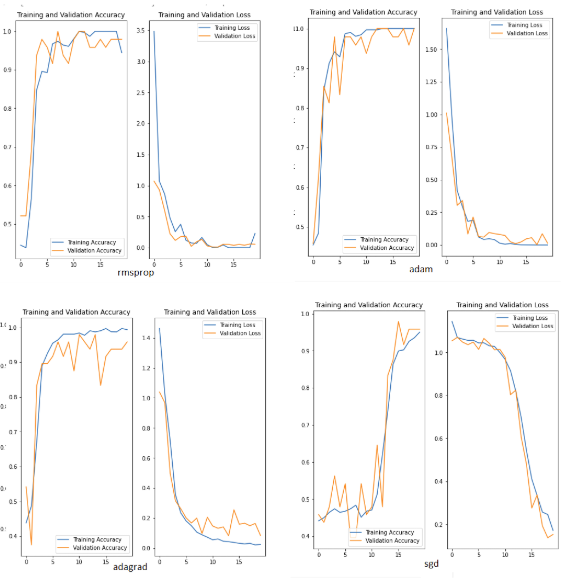
\includegraphics[scale = 0.8]{images_sav/exp2.png}}
\end{figure}

Заметим, что графики стали более волатильными - возросло количество потерь, упала точность, теперь тренировочная точность лежит в пределах от 93 до 100, а валидационная - от 87 до 100. Лучше всех себя опять показала модель с оптимизатором adam. 
